\section{Flutter}
	I pregi di Flutter sono numerosi e se ne vogliono citare alcuni. \newline
	Per primo si considera il linguaggio. Flutter viene sviluppato con il
	linguaggio (sempre appartente alla famiglia Google) Dart. Esso è
	multifunzione, può essere impiegato per lo sviluppo web (tant'è che è nato
	 per sostituire Javascript) e in tale linguaggio una variabile può sia
	presentare una tipazione statica a compile time, sia essere definita
	\textit{dynamic} e cambiare tipo più
	volte nel corso dell'esecuzione. Con Flutter basta scrivere una volta sola
	il proprio codice in Dart, e il framework penserà poi a creare i file
	necessari per essere eseguiti sia su iOS che su Android. Da qui ne segue un
	enorme risparmio di tempo e risorse, in quanto si dimezza il lavoro totale.
	Un altro aspetto importante è che
	grazie ad esso è possibile sviluppare in modo rapido, e ciò è permesso dalla
	funzione \textit{Hot Reload} che consente in qualche secondo di ricaricare
	la particolare sezione di codice che si sta testando senza dover ricaricare
	l'intera applicazione. In secondo luogo tale framework presenta
	facilitazioni notevoli relative al design degli elementi: con poche righe e
	senza essere esperti di grafica si può creare qualcosa dall'aspetto tutt'altro che
	banale. \'E doveroso accennare anche alle prestazioni: i \textit{widget}
	(elementi) di Flutter gestiscono automaticamente l'implementazione di
	funzionalità comuni quali lo scrolling, la navigazione, le icone e i
	caratteri in
	modo da rendere le performance del software paragonabili a quelle di app
	native sia su iOS sia su Android. 

	\subsection{Stateless e Statefull Widget}
	In Flutter esiste una prima importante distinzione fra widget diversi:
	quelli \textit{senza stato} e quelli \textit{con stato}. I primi possono
	anche essere chiamati widget statici, in quanto la loro forma non varia
	durante l'esecuzione. Nell'immagine \ref{stateless1}  viene mostrato un esempio di widget
	stateless. Innanzitutto bisogna importare il pacchetto
	\textit{flutter/material.dart} che contiene tutti i principali widget. Nel
	metodo main è presente solo una funzione, denominata \textit{runApp}, che
	ottenuto in input un widget con particolari caratteristiche, esegue sul
	dispositivo di test tale widget. Nell'esempio esso è chiamato MyApp ed
	estende la classe StateLessWidget. Un oggetto di questo tipo deve
	sovrascrivere il metodo \textit{build} che riceve in input il contesto nel
	quale l'app si trova (che consiste nel particolare valore delle variabili e
	di altri oggetti in quel preciso istante di esecuzione), e ritorna il widget
	vero e proprio che dovrà essere eseguito. Per ottenere una corretta
	struttura, anche in progetti più complessi di questo semplice esempio, è
	necessario introdurre la classe MaterialApp, e tramite il suo costruttore
	definire la sua \textit{home}, cioè la pagina principale, con una Scaffold,
	definibile come l'impalcatura del widget. \'E necessario introdurre nel parametro
	\textit{body} la classe che si vuole eseguire, la quale a sua volta estende
	StateLessWidget e presenta ancora il metodo build. Qui viene ritornato un
	widget che avrà posizione centrale (Center), sarà contenuto in un
	contenitore (Container, utile per decorare e aggiungere funzionalità a
	specifiche sezioni di codice), e mostrerà un testo con il più classico dei
	messaggi d'avvio (Hello World!). Questo widget non è interattivo, non
	cambierà mai graficamente e perciò si dice che non ha stato.
	 Da questo esempio si può già notare come la
	struttura del codice flutter assuma \textit{graficamente} un'indentazione
	naturale, con una gerarchia ad albero in cui c'è un padre iniziale e da cui
	seguono numerosi figli, padri di successivi widget.

	\begin{figure}[h!]
		\centering
		\begin{subfigure}{0.6\linewidth}
			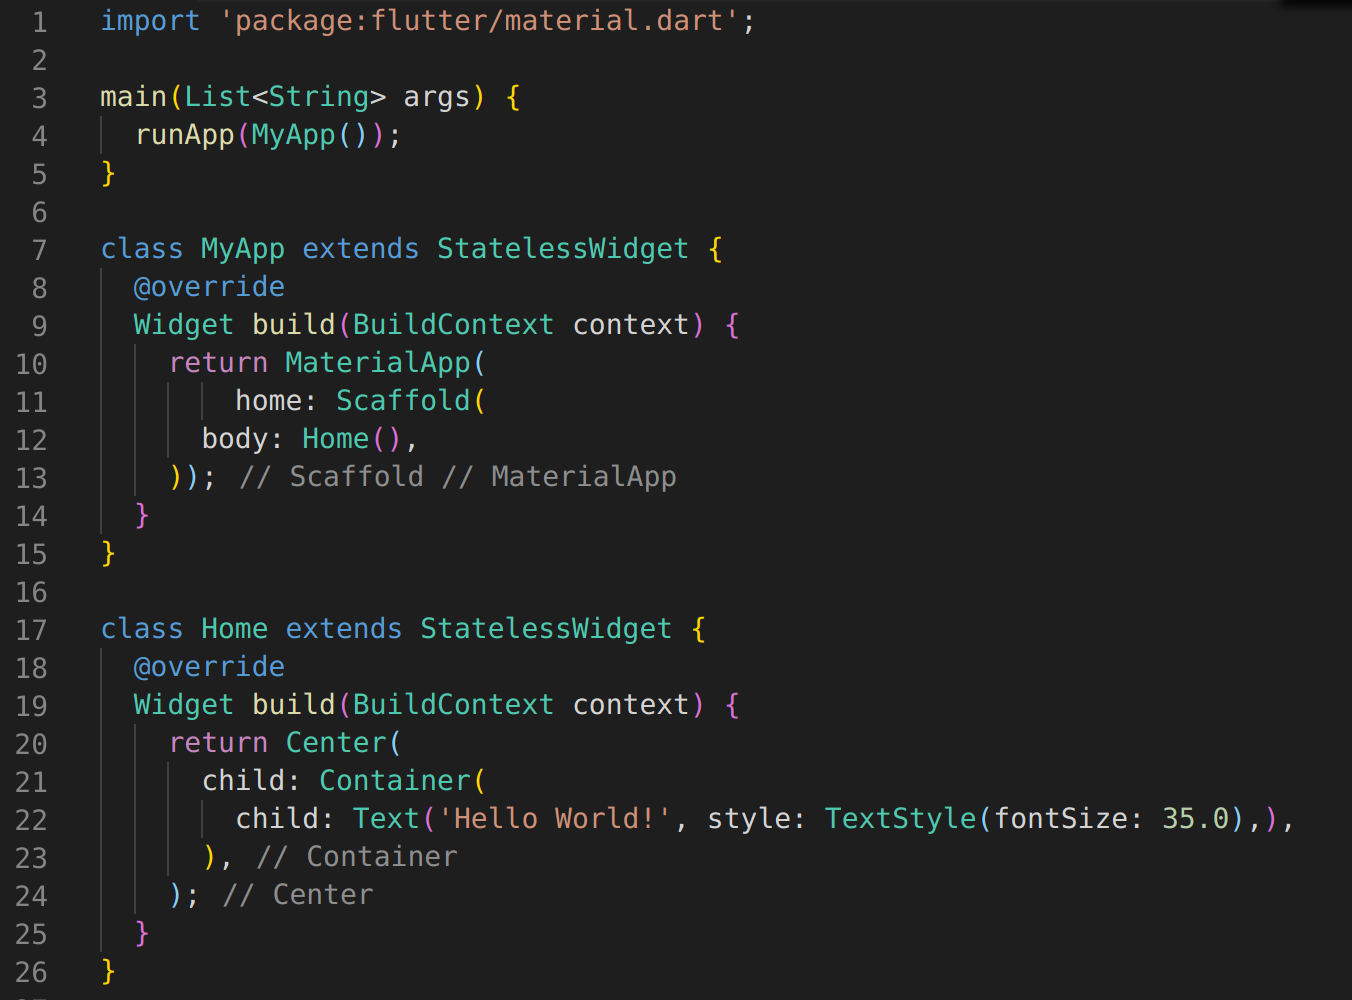
\includegraphics[width=\linewidth, height=7cm]{StateLessApp.png}
			\caption{Esempio di codice di widget stateless}
		\end{subfigure}
		\begin{subfigure}{0.3\linewidth}
			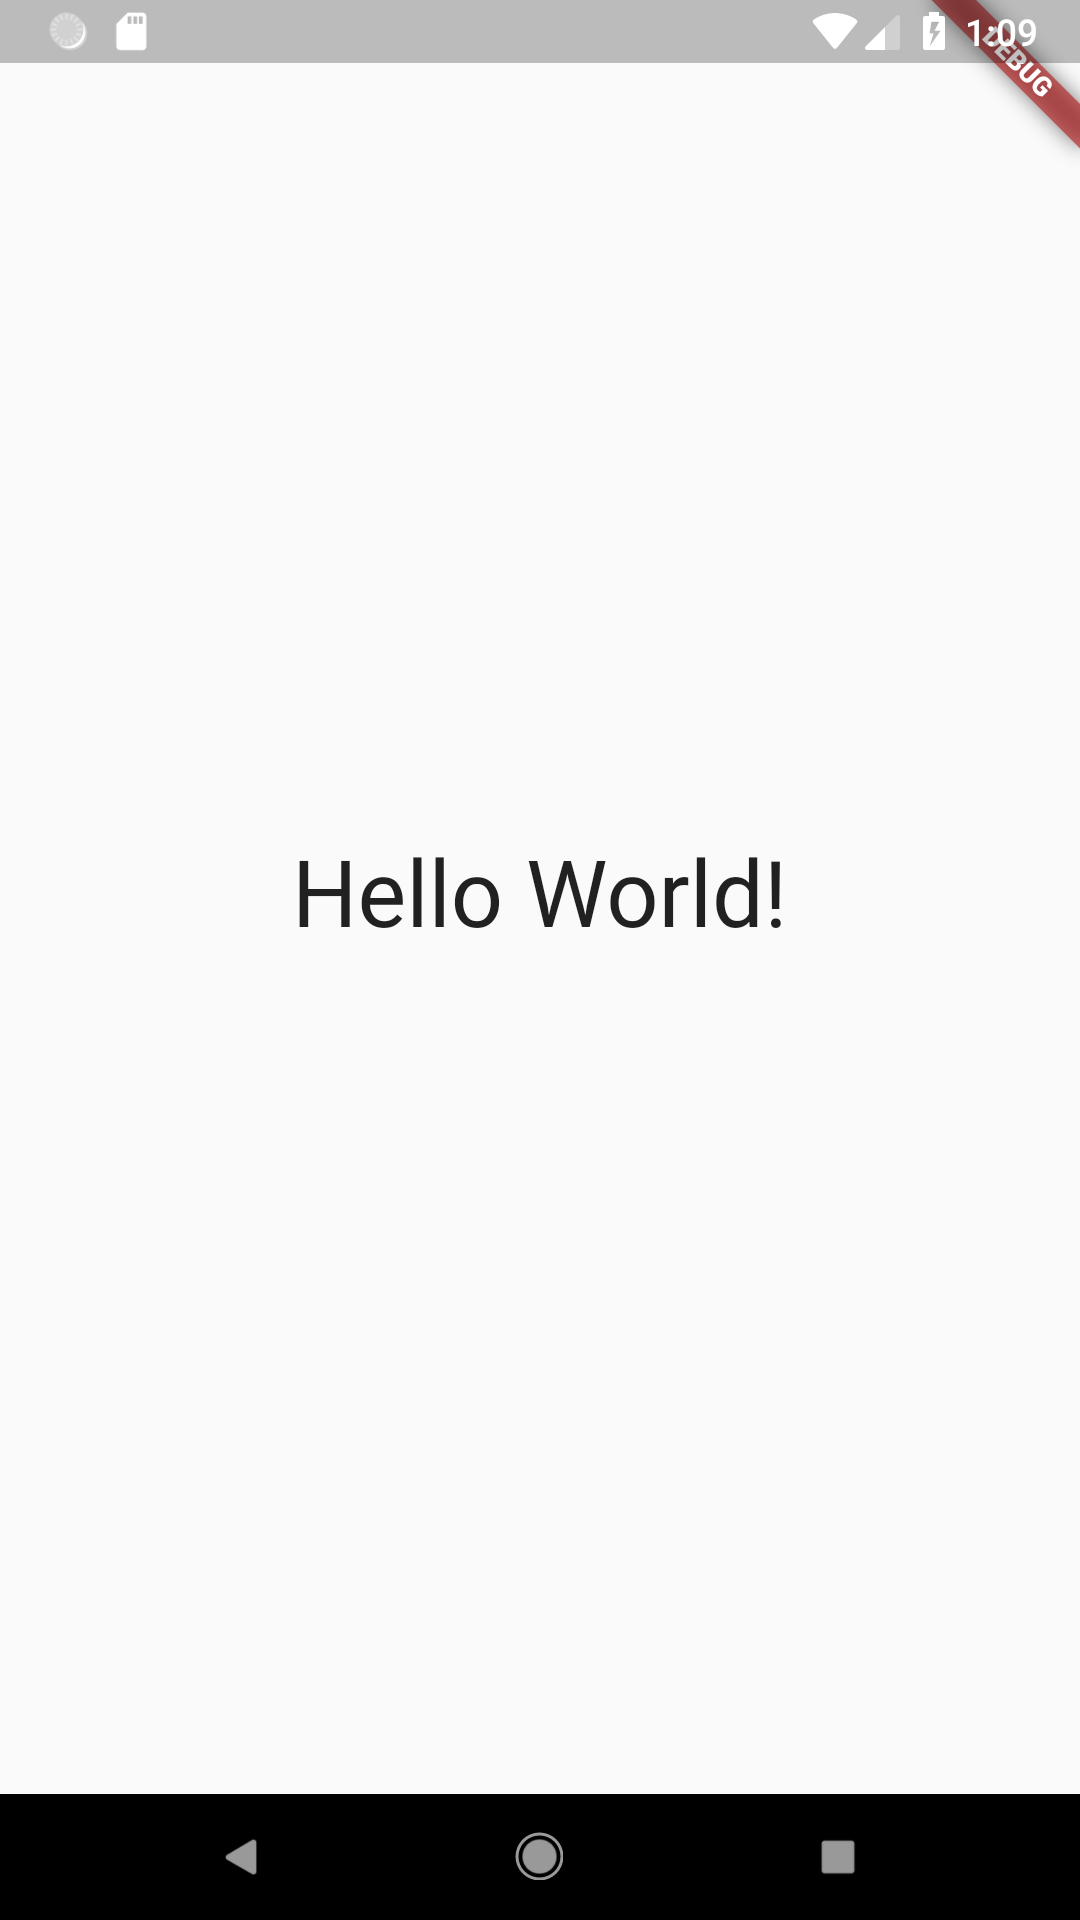
\includegraphics[width=\linewidth, height=7cm]{StateLessScreen.png}
			\caption{Risultato}
		\end{subfigure}
		\caption{}
		\label{stateless1}
	\end{figure} 

	Nell'immagine \ref{statefull} viene mostrato invece un widget di tipo
	Statefull. Si può notare come la prima parte del codice sia identica, con la
	classe MyApp che è ancora un widget senza stato. Ciò che cambia è la classe
	Home che ora è con stato e presenta un unico metodo sovrascritto chiamato
	\textit{createState}. La freccia =$>$ in dart è una notazione per scrivere in
	modo compatto un metodo che ritorna un unico oggetto, in questo caso una
	classe chiamata \_HomeState, che estende State$<$Home$>$. Il trattino basso
	in dart sta a indicare un oggetto privato, a cui quindi non è possibile
	accedere se non in quella specifica classe. \_HomeState possiede una
	varibile di tipo intero denominata counter (anch'essa privata grazie al
	trattino basso) e ha valore iniziale 0. Presenta poi un metodo denominato
	buttonPressed al cui interno risiede una funzione molto importante, la
	\textit{setState}. Quando viene compliata una sezione di codice che sta
	all'interno di tale funzione, viene richiamata la funzione build del widget
	in esecuzione ed è quindi grazie ad essa che l'app diventa interattiva, in
	quanto tramite azioni dell'utente cambiano i valori delle variabili.
	Nell'esempio è presente un pulsante (FloatingActionButton) che aumenta il
	valore della variabile counter, che viene stampato a schermo. Da notare
	infine come si possa accedere al metodo toString di un oggetto in dart
	anteponendo al suo nome il carattere \$.

	\begin{figure}[h!]
		\centering
		\caption{Esempio di codice di widget statefull}{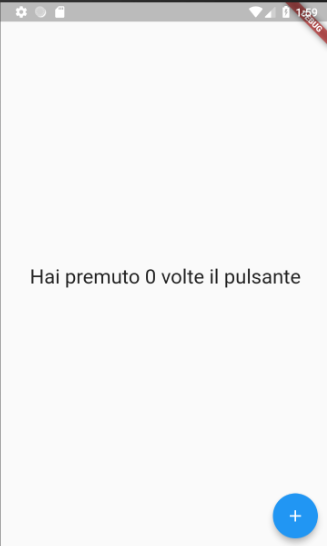
\includegraphics[scale=0.35]{StateFullApp.png}\label{statefull}}
	\end{figure}

	\subsection{Principali Widget}
	Di seguito vengono riportati i widget di cui si è fatto maggiore uso
	all'interno dell'applicazione.
	
	\begin{trivlist}
		\item \textbf{Text} \newline
		Questo widget permette di mostrare a schermo le stringhe fornite come
		primo argomento al suo costruttore (\verb|Text("Testo da mostrare")|).
		Il testo può svilupparsi su più righe o su una sola a seconda delle
		costanti di layout della particolare schermata nella quale risiede il
		widget. Nel costruttore possono essere indicati diversi argomenti
		opzionali, tra cui lo stile. Se si vuole indicare un particolare stile
		al proprio testo bisogna inserire un TextStyle, cioè un'ulteriore classe
		che gestisce il font, l'inserimento del grassetto o del corsivo e la
		formattazione dell'intero testo (giustificato, allineato a sinistra o a
		destra e centrale).  
		\item \textbf{Row, Column} \newline
		Questi widget vengono spesso utilizzati per ottenere schermate ordinate
		e gradevoli dal punto di vista estetico all'utilizzatore. Il parametro
		principale di entrambe è l'argomento \verb|children| (e non \verb|child| come
		spesso accade per altre classi), proprio perchè sono pensati per
		contenere diversi widget disposti rispettivamente in orizzontale o in
		verticale. La loro grandezza in pixel sarà formata dalla somma della
		dimensioni di ciò che contengono e si possono ancora una volta inserire diverse
		preferenze di stile come la posizione rispetto all'asse principale o
		secondario. 
		\item \textbf{Stack} \newline
		\'E simile ai due precedenti in quanto anch'esso contiene diversi widget
		figli. Se ne differenzia in quanto non privilegia un'unica direzione di
		posizionamento, ma si può indicare per ogni figlio la posiziona esatta
		in pixel che dovrà avere sullo schermo. Questo passaggio viene
		effettuato racchiudendo il widget che si vuole inserire all'interno di
		un'istanza della classe Positioned (che sarà uno dei figli dello Stack)
		e indicando gli esatti pixel nel suo costruttore. 
		\item \textbf{Container} \newline
		Crea un elemento rettangolare che avrà come altezza e lunghezza le
		minime dimensioni per poter contenere il widget indicato come child. \'E
		molto utilizzato nel momento in cui si vuole migliorare graficamente una
		schermata in quanto tramite il parametro opzionale decoration si può
		introdurre una nuova classe chiamata BoxDecoration che gestisce un
		grande insieme di aspetti grafici come i contorni (angoli e
		ombre) o riempire con un colore o un'immagine il Container.
	\end{trivlist}

	\subsection{Material Design}
	Il Material Design è un linguaggio visuale che unisce i classici principi di
	un buon design con l'innovazione della tecnologia e della scienza. 
	\cite{material} \newline
	Tale design è interamente sviluppato da Google e fa uso di layout basati su
	una griglia, animazioni e transizioni. Sono
	
